\chapter{Metodology}
\label{chap:Metodology}


\section{System Model}
\label{sec:control_model}

ilustramos o processo com a Figura \ref{fig:control_model_fig}. 

\begin{figure}[thpb]
  \centering
  \resizebox{150mm}{!}{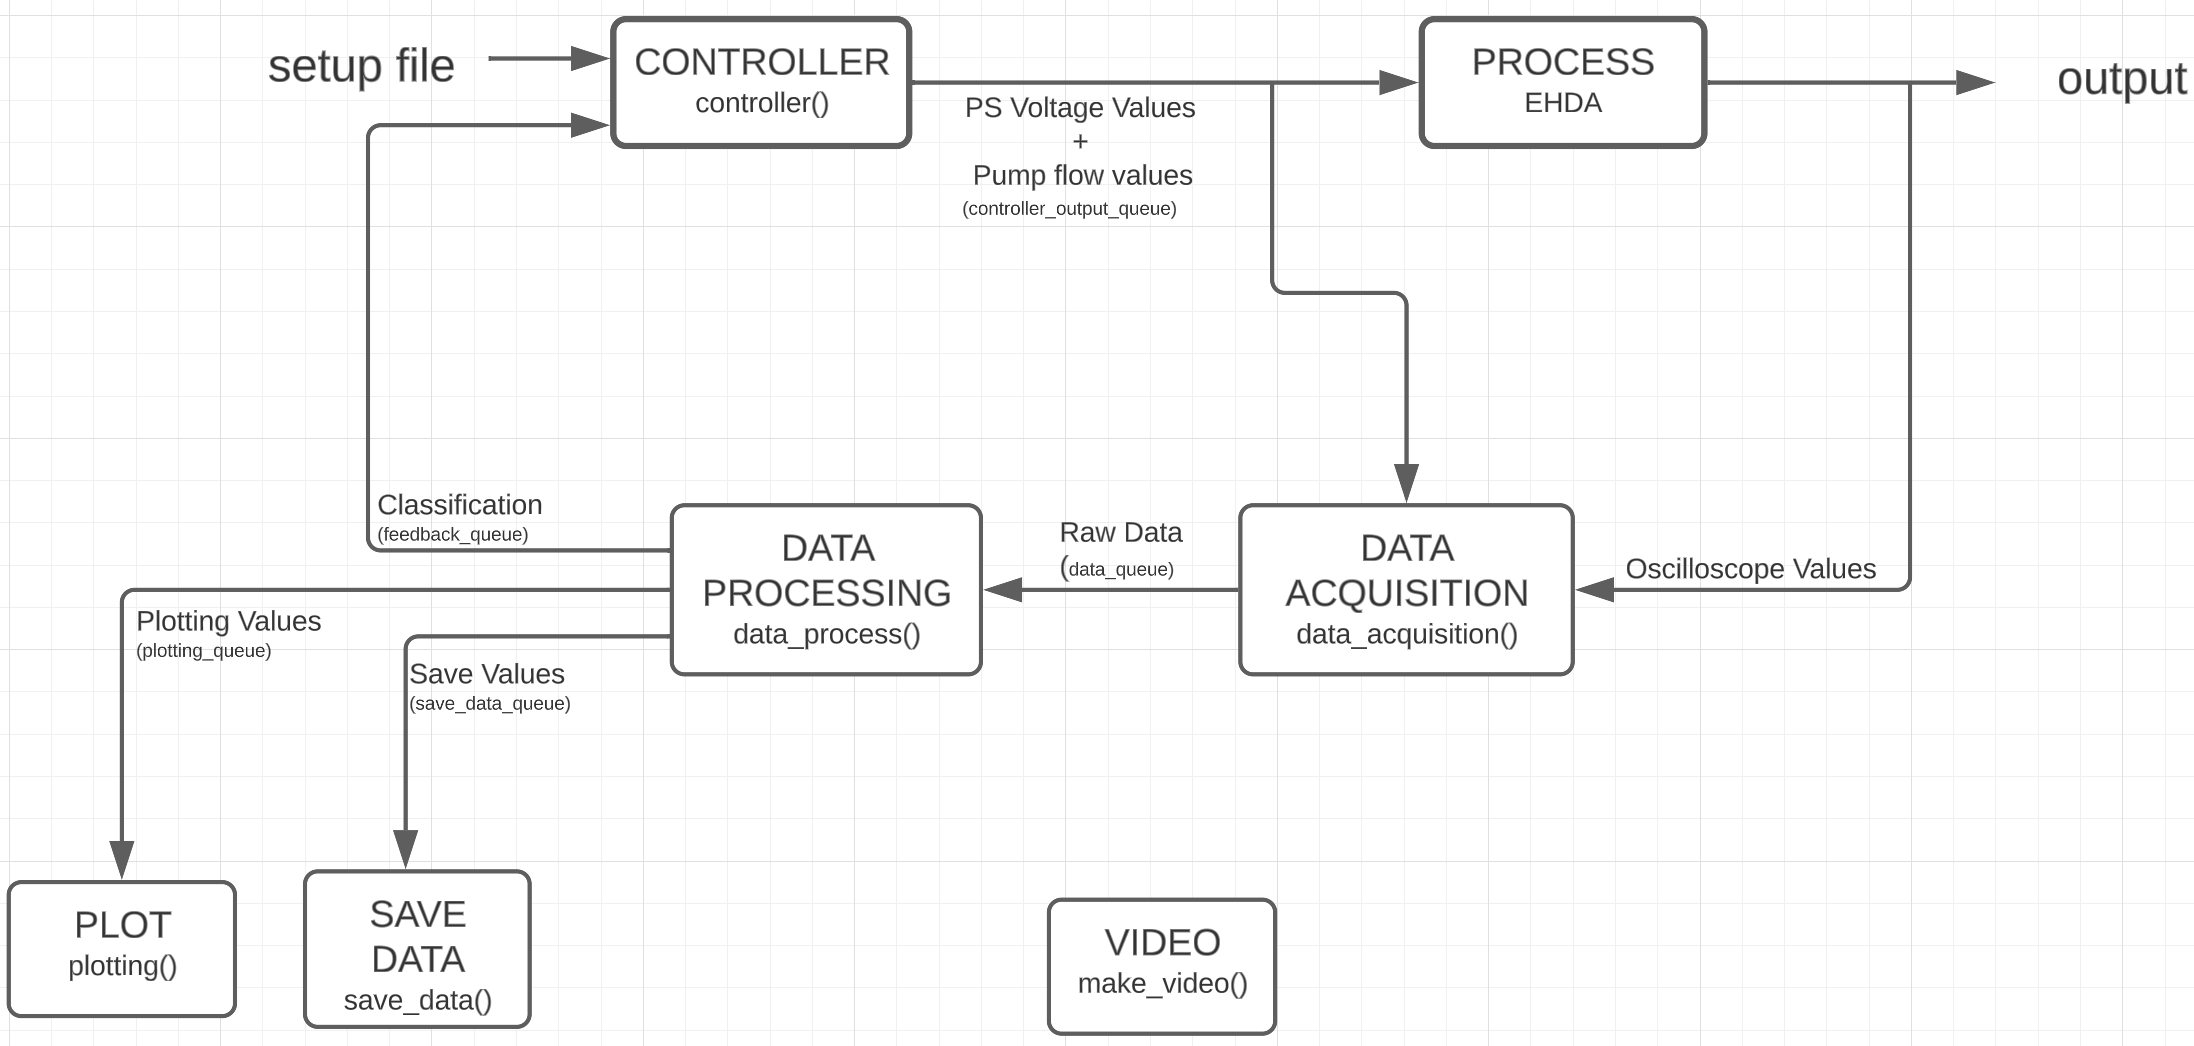
\includegraphics{Figuras/control_loop.png}}
  \caption{EHDA automation system setup}
  \label{fig:control_model_fig}
\end{figure}

\section{Threading and Queues}
\label{sec:concurrency}

    In order to implement this system model to the software and explore parallel processing each system in the
    model was developed as a separate Thread. For cuncurrency purpose and the flux of data in the control cicle was used queues structures.
    
    \begin{enumerate}[a)]
        \item Item 1;
        \item Item 2; 
        \item Etc.     
    \end{enumerate}

\section{Classification}
\label{sec:section_classification}

\subsection{Statistical Analisys}

 According to \cite{Sjaaks} evaluating the current data flowing through the nozzle to the plate we can analyze the signa that represents the spraying dynamics.
 through statistical analysis in this signal such as mean value and standart deviation we can analyze if the signal is stable or not.

 Our classification by statistical analysis was implemented in the automation library made by the previous student \cite{Monica}.

 Each current sample is 0.5s of current data in 10kHz sampling frequency.
 By the processing thread we take this sample and evaluate the followings statistical values.
        
        - Sjaak Classification -> Classifies Dripping, Intermittent and Cone Jet
        
        - Monica Classification -> Classifies Corona Sparks

        - João Classification -> Classifies Multi Jet

	The algorithm implemented works in the following way:
	\begin{algorithm}
        \caption{Statistical Classification}\label{alg:statistical_class}
        \begin{algorithmic}
        \Function{statistical\_classification}{$sample$} 

            \State $spray\_mode \gets "Undefined"$;
            \State $mean \gets sample.mean$; 
            \State $std\_deviation \gets sample.std\_deviation$;
            \State $median \gets sample.median$;
            
            \If{ $mean / std\_deviation$ > 2.5}
                \Comment{Sjaak classification \cite{Sjaaks}} 
                \State $spray\_mode \gets "Dripping"$;
            \ElsIf{$ 2.5 < mean / std\_deviation < 2.5 \And mean / std\_deviation > 0.3 $}
                \State $spray\_ mode \gets "Intermittent"$;
            \ElsIf{ $mean / std\_deviation$ < 0.3}
                \State $spray\_ mode \gets "Cone Jet"$;
                \State $cone\_jet\_mean \gets mean$;
            \EndIf

            \If{ $mean / std\_deviation$ > 2.5}
                \Comment{Monica classification \cite{Monica}} 
            \EndIf

            \If{ $spray\_mode == "Cone Jet"$}
                \Comment{João classification} 
                \If{ $cone\_jet\_mean > 1.14 \times mean$}
                    \State $spray\_ mode \gets "Multi Jet"$;
                \EndIf
            \EndIf

            \Return $spray\_ mode$;
        \EndFunction
        \end{algorithmic}
    \end{algorithm}


\subsection{Machine Learning}


\section{Routine Sequences}
\label{sec:routine_sequences}

    The software was previously developed as a electrospray multipurpose library\cite{Monica}. 
    Continuing this methodology, in the setup json file there is a "sequence" atribute which can chosen beetween "ramp", "step", "map" or "control".
    The controller thread will manage what the algorithm must do for each sequence.

\subsection{Ramp}



\subsection{Step}


\begin{algorithm}
    \caption{STEP sequence in controller thread}\label{alg:stepping_algorithm}
    \begin{algorithmic}
    \Procedure{STEP}{$voltage\_start,voltage\_stop$} 
        \State $voltage \gets voltage\_start$
        \While{$voltage \leq voltage\_stop$} \Comment{scanning voltage range}
            \State \Call{send\_voltage\_command}{voltage}
            \State \Call{sleep}{step \_time}
            \State $voltage \gets voltage + step\_size$
        \EndWhile
    \EndProcedure

    \end{algorithmic}
\end{algorithm}

\subsection{Map}

    \begin{figure}[H]
        \center
        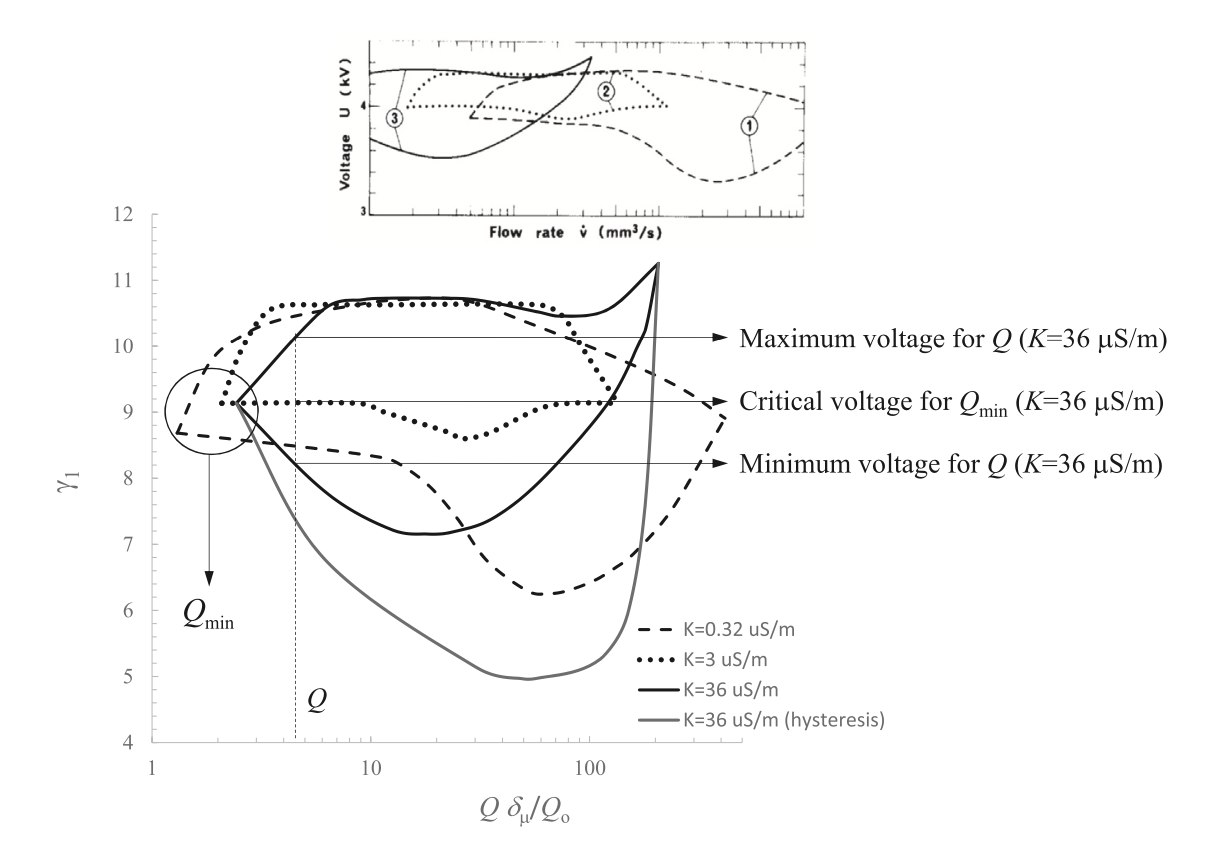
\includegraphics[width=13cm]{Figuras/ganan_calvo_map.png}
        \caption{Domains of existence (stability) of Taylor cone-jets. \cite{gananCalvo} }
        \label{fig:ganan_calvo_fig}
    \end{figure}


    \begin{algorithm}
        \caption{MAP sequence in controller thread}\label{alg:mapping_algorithm}
        \begin{algorithmic}
        \Procedure{MAP}{$flowrate\_values$} 
            \ForAll{flowrate\_values}  \Comment{scanning in the flowrate range}
                \State \Call{send\_flowrate\_command}{flowrate}
                \State $voltage \gets voltage\_start$
                \While{$voltage \leq voltage\_stop$} \Comment{scanning in the voltage range}
                    \State \Call{send\_voltage\_command}{voltage}
                    \State \Call{sleep}{step \_time}
                    \State $voltage \gets voltage + step\_size$
                \EndWhile
            \EndFor
        \EndProcedure

        \end{algorithmic}
    \end{algorithm}

    In the figures 5 and 6 we can see the results of this mapping experiments. The liquid used is pure ethanol. 
    Each figure has 3 graphs with shared x axis representing the samples collected. The first is the current values collected through all the experiment.
    The second is the voltage values applied in each window of data collected. The colors represent the spraying classification defined by our routine.
    The third graph shows the current mean value of each data sample.
    Note that the experiment is composed of loops that increase voltage, change flowrate and repeat.


    \begin{figure}[H]
        \center
        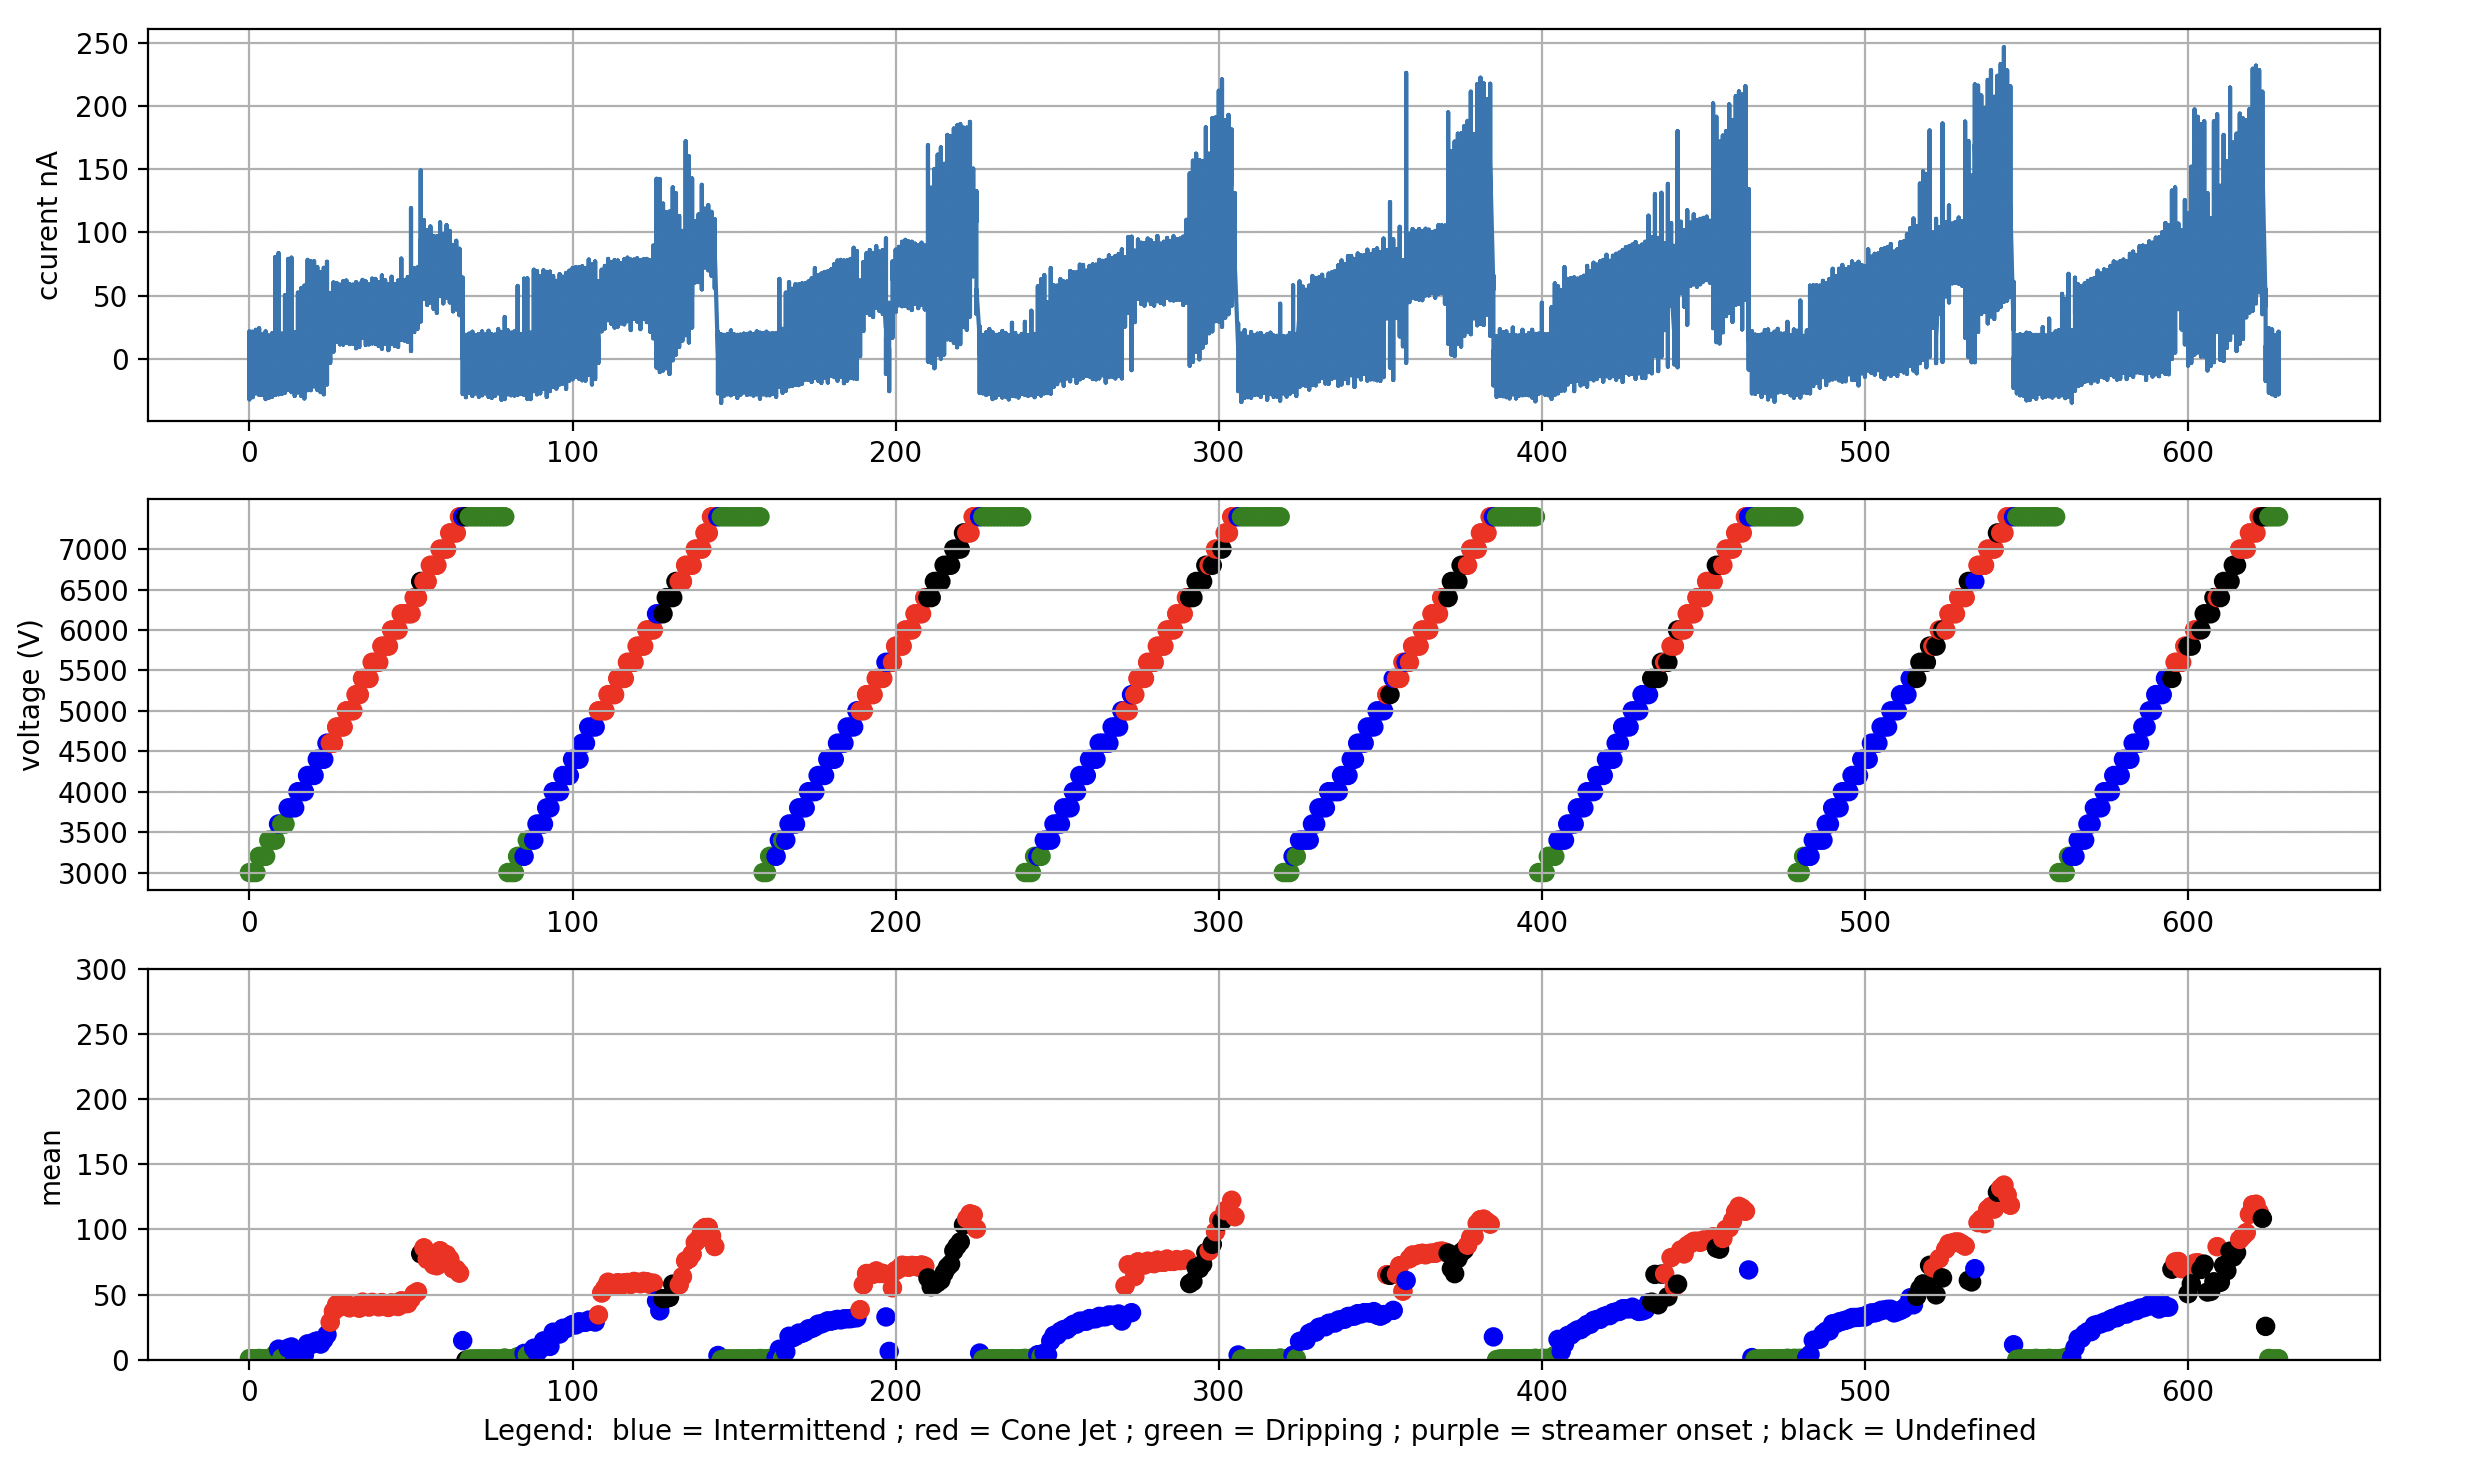
\includegraphics[width=15cm]{Figuras/report2/map2Data.png}
        \caption{Mapping Experiment example 1}
        \label{fig:map2Data_fig}
    \end{figure}


    \begin{figure}[H]
        \center
        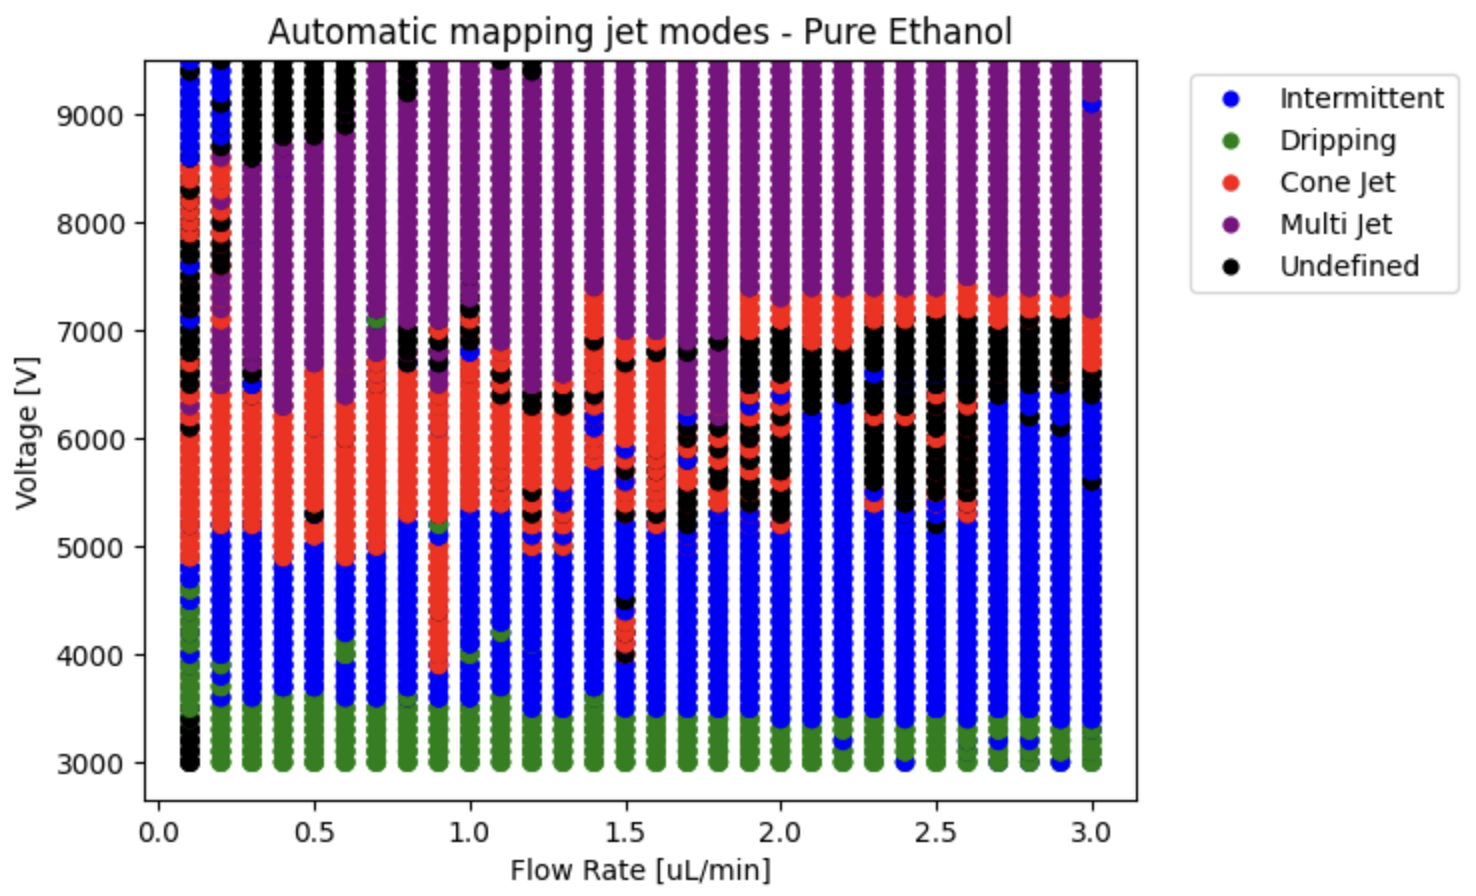
\includegraphics[width=15cm]{Figuras/report4/map-2023-03-02.png}
        \caption{Mapping Experiment example 1}
        \label{fig:map3Data_fig}
    \end{figure}



\subsection{Control}

\section{Optimizations}
\label{sec:routine_optimization}

About the python algorithm to turn the experiment autonomous it was made a study and modelling of the software architecture to optimize it for further control loop application to be implemented. From the changes made until now it highlights:

- Integrate high speed camera to the experiment routine.

- Remodel the software to support threads in order to separate the sensoring and controlling routines.

- Reduce the data collected size.

- Synchronize the power supply step commands and voltage sensoring.

- Reestructure the setup file in order to make it more intuitive to use the experiment.

- Improvements in code organization and readability.

About the setup,integrate was changed the liquid, nozzle diameter and distance to the plate in order to
make the experiment the most stable and easy to reach cone-jet mode as possible. For example, while doing experiments we discovered that the frequency of the pump machine internal motors was creating an interference in the flowrate. Therefore compromising the stabilization in cone jet mode. A solution for that was to increasethe flowrate wich smooths this pumping noise. For that was also necessary to increase the nozzle diameter to balance with all other variables from the experiment.

\subsection{Pump Integration}

    The pump integration in the automation algorithm bring us a new controllable variable, the Flowrate. Now we can control the spraying mode with the
    two main variables that afect the system. 
    It will bring more complexity for the system since now we are dealing with multivariable control.
    Controlling also the flowrate gives to this project a new dimension in the system giving us freedom to explore the flowrate properties.
    % Our control model is now a MISO \footcite{MISO: Multiple Inputs Single Output} system. The crossover (couple) between the controlled variables will be evaluated in further reports.

    About the pump interface. As I could not find a good ready-to-use library for this pump I developed an simple and intuitive interface to be our software routine.
    The communication protocol used is RS-232. In the software routine the communication used is python serial interface. The pump commands list were found in the user manual.



\clearpage